% !TEX root =  main.tex
\section{Open-domain Event Schemas}
\label{sec:schemas}
Our approach builds on our preliminary work for generating schemas. The key premise behind our approach is that we can aggregate information about types of events from specific event mentions through appropriate generalization and important information about events (i.e., the participants and their roles) are often co-mentioned. Accordingly we gather frequently co-mentioned entities and relations to capture typical participants and their roles within the schema. This corpus-driven approach can discover event schemas that cover a broad range of domains mentioned within the corpus. 

Figure~\ref{fig:schema-generation} shows the architecture of our system developed based on this premise. 
\begin{figure}[htbp]
\vspace{-2ex}
\begin{center}
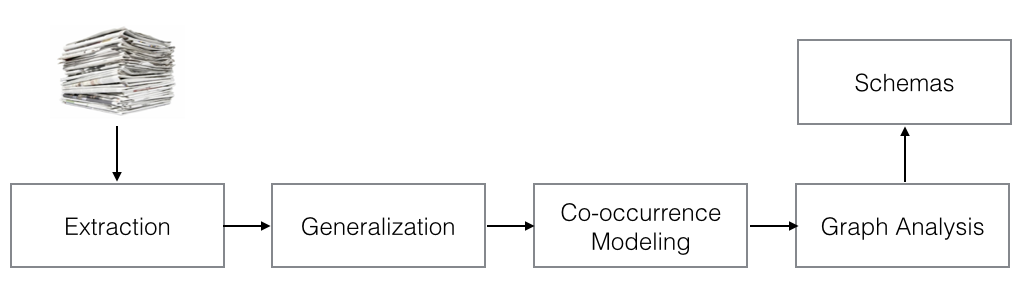
\includegraphics[height=1.75in, width=5.25in]{figures/schema-architecture}
\vspace{-4ex}
\caption{\label{fig:schema-generation}Schema Generation Pipeline}
\end{center}
\vspace{-2ex}
\end{figure}
Starting from a large collection of stories we first extract a generalized representation of the event mentions in the text. 
We do this by first processing the documents using an Open IE system(e.g. \cite{mausam-emnlp12}) and the generalize the specific extractions into generalized relations by assigning types to the arguments. Then, we compute the co-occurrence statistics between the generalized mentions. Next, we identify relations to seed schema generation. We then construct a relation graph starting from the seed, and use graph analysis algorithms to identify the relations that belong to the schema. As a final step we resolve co-referring entities and relations and output the schema. There are several fundamental challenges in all stages of the pipeline. In this section, we will detail the challenges and the directions that this project will investigate for each stage.
%We use a richer representation, design techniques for generalizing arguments to an appropriate level, investigate graph-based formalisms that can effectively model sense and topic-drift issues during clustering, and build a learning-based approach for effectively scoring the generated schemas.
 
\subsection{Representation}
%The first stage in our pipeline involves extracting and representing event mentions from text. 
Using extractions to represent information in sentences is lossy. On the other hand retaining all information in a sentence doesn't scale well. Previous automatic approaches used extremely limited context to represent events using (subject, verb) and (verb, object) pairs (e.g., Chambers and Jurafsky, 2009). Using such limited representations mitigate sparsity but lead to incoherent schemas which mix distinct events. Also, even with a more specific representation, such as an (arg1, relation, arg2) triple, is still close to the source text and raises two fundamental sparsity problems: 1) Using specific mentions of events doesn't provide any generalization power. 2) Syntactic and lexical variability can mislead the system into treating the different mentions of the same event as separate events. 
%Our preliminary work showed that one of the fundamental challenges in learning schemas from text is the context vs. sparsity trade-off in representation. On the other hand, capturing more context using entire relation triples of the form (arg1, relation, arg2) leads to improved results. However, w

\subsubsection{Extraction}

To address these challenges, we propose to explore the combination of Open IE extractions with semantic role annotations. Semantic roles present a nice intermediate between ontology-free Open-IE and tight semantic ontology in closed IE systems. The thematic roles sought by SRL systems are general purpose roles that apply to a wide variety of relations. The key advantage with semantic roles is that unlike Open IE arguments, semantic role assignments are not susceptible to simple syntactic transformation and because the arguments are thematic roles, it is easy to encode N-ary relations compactly. We plan to use an existing semantic role labeling system off-the shelf (e.g., Clear SRL~\cite{punyakanok2008importance}).

\subsubsection{Generalization}

Extractions yield information about specific mentions. Generalizing from these specific mentions is the key step in extracting knowledge about types of events. This involves mapping specific instances (e.g., Barrack Obama) to an appropriate class (e.g., US President). This immediately raises two basic questions: 1) What is the underlying ontology of classes? 2) How does one map the arguments and relations to the appropriate class? Depending on the relation {\em Barrack Obama} may map to a {\em US President}, {\em Senator}, or {\em Person}.  

In this work, we will target fine grained semantic types by leverage existing resources such as Freebase, NELL and WordNet for assigning semantic types to arguments and relations. Freebase is a crowd-sourced and curated knowledge base that contains more than 43,000 types (i.e., classes)~\footnote{as of September 1st, 2014.}. Entity classification systems~\cite{ling2012fine}, entity linking systems~\cite{lin2012no}, and relation extraction systems~\cite{hoffmann-acl11,hoffmann-acl10} have been developed to identify instances of Freebase types. These provide a great starting 
point for mapping named entities and some subset of relations into Freebase. Events also involve common noun arguments (e.g, The fire burned down {\em the entire condominium} in 2 hours.). It is important to be able to generalize {\em condominiums} to its class {\em building}. We use Wordnet type hierarchy to assign classes to common nouns.
Determining the appropriate level of generalization is a difficult problem. In our preliminary work we created multiple entires one for each type in the hierarchy up to the root. In addition to being inefficient, this method cannot be tuned to select a desired level of generalization. We propose to investigate prior work on selectional preferences~\cite{ritter2010latent} and class models~\cite{clark2000class} to determine the appropriate class assignment given an extraction.
 
 \subsection{Schema Generation}
The main intuition behind schema generation is that frequently co-mentioned relations belong to the same schema and contain the salient entities and their roles.  As we alluded to earlier, not all stories about an event type will mention (or necessarily) have the same set of sub-events or entities. For example, not all lawsuits will be decided in favor of the defendant and not all lawsuits will involve the filing of briefs from friends of the court, and in some cases the story itself may omit its mention. By gathering co-mentioned relations from pairwise co-occurrence models, we implicitly allow for the aggregation of information that may sometimes be missing. 

\subsubsection{Modeling Relation Co-occurrence}

We gather frequently co-mentioned relations from the pairwise co-occurrence model. In our prior work, we developed {\em Rel-grams} a relation co-occurrence model, which estimates the co-occurrence probabilities of generalized event mentions. We will follow the template in our preliminary work on Rel-grams generation to produce a large table of co-occurrence frequencies and evaluate standard conditional probability estimation techniques and approaches for combining estimates obtained over different windows of document level co-occurrence. The key implementation challenge here is scaling to large collections. Rel-gram computation involves counting items that are linear in the size of the collection\footnote{With a constant proportional to the square of the average size of a document.}. We will leverage the many Map-Reduce implementation optimizations that we developed for our preliminary work.

\subsubsection{Graph Analysis}
The are two main challenges in building schemas: 1) Identifying useful seeds or starting points for schemas, and 2) Effectively selecting relations to include in a schema.

\textbf{Seeding Schemas} 
The pairwise co-occurrences represent a large graph where the generalized relations are nodes and co-occurrences specify edge weights. In this setting, a direct approach to gathering co-mentioned relations is to perform clustering over this graph (either bottom-up or top-down). Instead we propose to investigate a seed-based expansion approach, which has several key benefits: a) Avoids the problem of large clusters resulting from hub nodes that are general purpose relations (e.g., {\em father of}, {\em spokesperson for}). b) Allows local structure around nodes to govern the inclusion in schema, which makes it easier to design selection algorithms.  c) Allows for an on-demand clustering of graph given any starting point. As we will point out later this flexibility is desirable for both development purposes (control for the seeds), as well as for use in applications which can provide an effective circumscription of the graph based on their input.

We propose to explore a probabilistic generative model for seed selection. Given a co-occurrence model with appropriate probabilistic semantics, we can directly construct a generative probabilistic model, which specifies the probability of observing other relations having observed a specific relation. The quality of a seed can be approximated by the quality of the distribution governing its neighborhood (e.g., perplexity of observing the neighboring nodes). selecting seeds that cover diverse events, as well as providing strong anchors for building schemas. 

\textbf{Graph Analysis} 
We propose to investigate principled approaches for selecting the relations to include in a schema. 
The neighborhood of a seed relation is a directed weighted graph. The problem of selecting the best of nodes around the seed is a classic reachability problem that can be formulated in many ways.  Based on our preliminary work, we identify two main challenges that an effective formulation should address: 1) Prune relations that are overly general and occur in many scenarios, and 2) Avoid topic and sense drift.   

To this end, we propose to investigate graph-based formulations that leverage both properties of the graph as well as lexical properties about the relations. Graphical properties such as weights on the edges, connectivity of the nodes, and connectivity to the seed (or other central relations) all provide valuable information in detecting overly general relations, which co-occur with many other relations. Lexical distributional similarity measures (e.g., word2vec similarity) over the generalized relations, and context models of the top entities can also provide useful information to detect topic drift.  

The graphical properties such as the weights on the edges, the connectivity of the nodes, and the connectivity to the seed (or other central relations) can all be used as features.
We propose to investigate methods that specifically address the topic-drift issue. In addition to the graph structure induced by the co-occurrence model, we will also investigate methods that can use the lexical similarity between the relations can also be used to detect topic drift. Prior approaches have addressed a similar sense-drift issue in translations~\cite{soderland2010panlingual}. Recent graph-based approaches such as~\cite{lao2011random,gardner2013improving} also show promise for the viability of graph-based approaches to combine multiple types of features. 

\textbf{Creating Slots} To output a schema, we resolve entities and relations that are co-referent and output the result as participants. We will rely on existing co-reference systems (e.g. Stanford Co-reference~\cite{lee2011stanford}) to provide co-reference. At this stage we can to some extent also recover from co-reference errors if they end up resulting in merging entities with incompatible types. Similar intuitions have been successful in recent approaches for joint entity linking and co-reference resolution~\cite{hajishirzi2013joint}. The final step is to produce a label on the participants. We will explore alternatives for labeling using some simple generalizations on the the top instances seen for each participant. 

%Lastly, we also develop a scoring mechanism. Following Open IE approaches, we will develop a learning-based approach that uses yuma

\subsection{Contributions}

In this phase, we propose to design a representation that leverages existing large scale resources, use scalable  techniques that combine open information extraction with semantic role labeling, and develop principled graph-based solutions for identifying seed relations, and constructing schemas. Upon successful completion, the key contributions of this phase will include:
\begin{itemize}[noitemsep,nolistsep]
\vspace{-1ex}
\item An effective representation that includes adequate context to reduce ambiguity. 
\item Generalization techniques that address sparsity. 
\item Graph-based approaches that leverage graphical properties to address topic-drift. 
%\item Scalable method for effectively scoring generated schemas. 
\end{itemize}

